\documentclass[../main.tex]{subfiles}

\begin{document}

\section{Results}

\subsection{Fashion-MNIST}
\subsubsection{CNN}
The training session for the CNN on the Fashion-MNIST dataset initially developed promisingly. However, the loss shown in the validation set quickly increased in the last epochs, as shown in figure \ref{fig:fashion_mnist_cnn_history}

\begin{figure}[H]
    \begin{subfigure}{.5\textwidth}
        \centering
        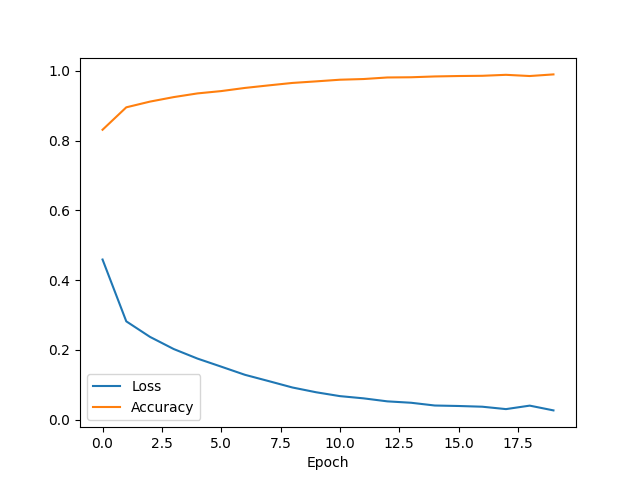
\includegraphics[width=1.1\linewidth]{assets/fashion_mnist_train_history.png}
    \end{subfigure}
    \begin{subfigure}{.5\textwidth}
        \centering
        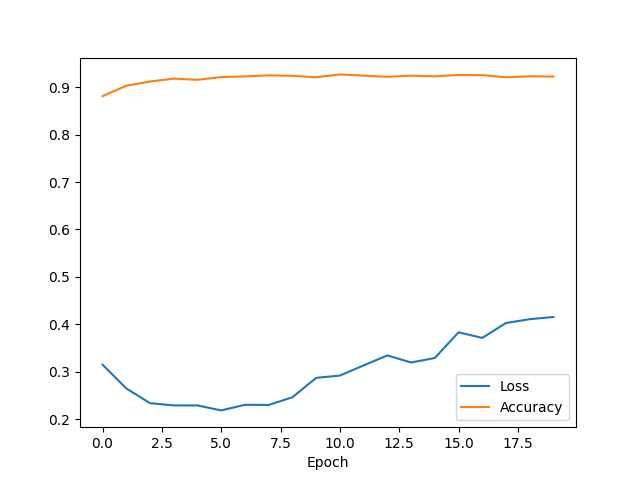
\includegraphics[width=1.1\linewidth]{assets/fashion_mnist_val_history.png}
    \end{subfigure}
    \caption{History of loss and accuracy of the training and validation set as they develop through the epochs.}
    \label{fig:fashion_mnist_cnn_history}
\end{figure}

After modifying the network structure by implementing dropout in the model, the validation accuracy and loss progressed nicely and as expected. This is shown in figure \ref{fig:fashion_mnist_cnn_dropout_history}

\begin{figure}[H]
    \begin{subfigure}{.5\textwidth}
        \centering
        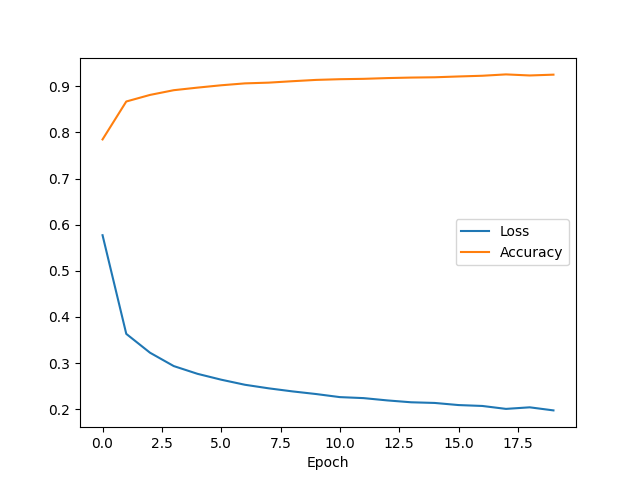
\includegraphics[width=1.1\linewidth]{assets/fashion_mnist_train_history_dropout.png}
    \end{subfigure}
    \begin{subfigure}{.5\textwidth}
        \centering
        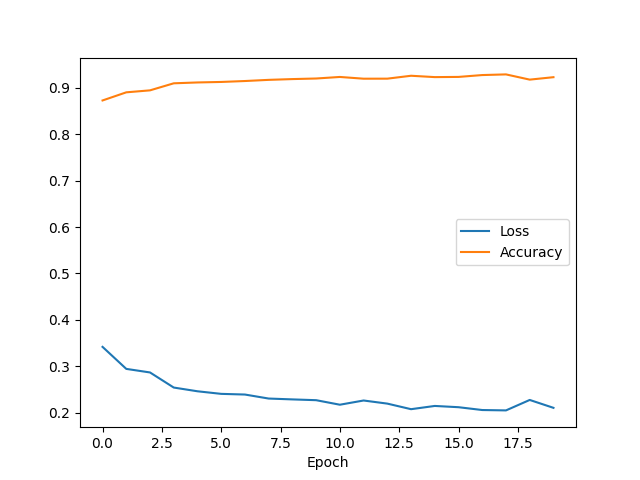
\includegraphics[width=1.1\linewidth]{assets/fashion_mnist_val_history_dropout.png}
    \end{subfigure}
    \caption{History of loss and accuracy of the training and validation set as they develop through the epochs. Here, dropout is implemented into the model.}
    \label{fig:fashion_mnist_cnn_dropout_history}
\end{figure}

After evaluating the model on the test set and comparing against the real values, the accuracy on never before seen data is $92\%$ (this result can be reproduced by running \verb|src/fashion_mnist/predict.py|). In figure \ref{fig:cnn_fashion_predictions}, we see a small selection of test data, the predicted category and the actual category.

\begin{figure}[H]
    \centering
    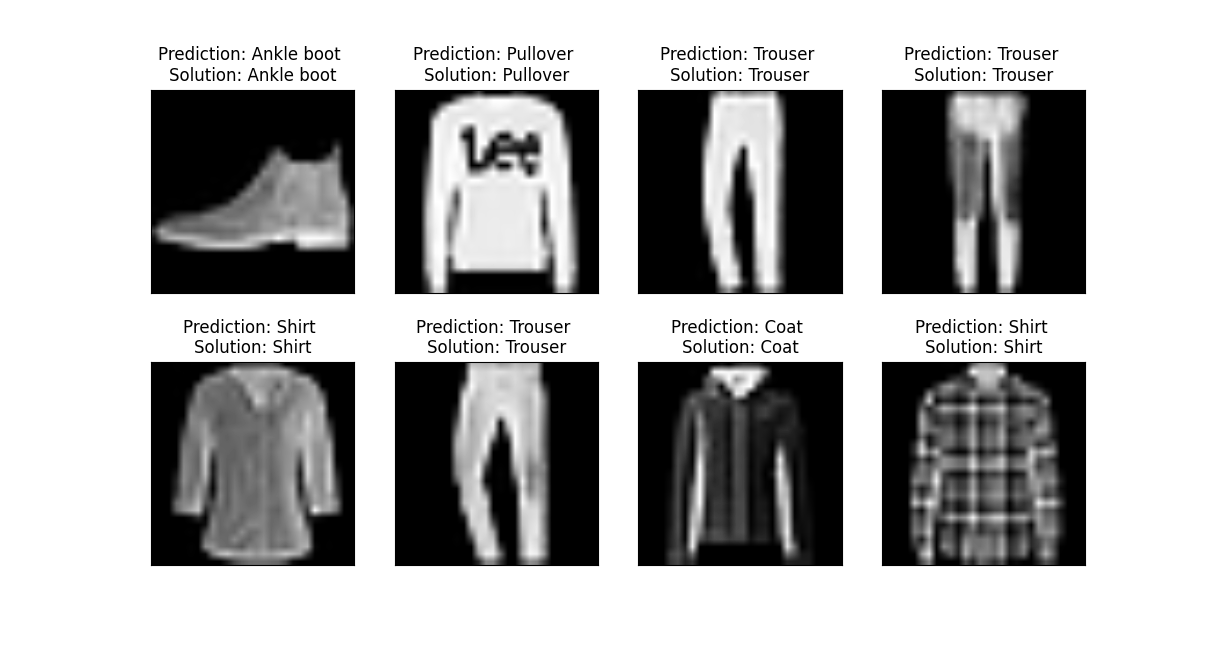
\includegraphics[width=\textwidth]{assets/cnn_fashion_predictions.png}
    \caption{A small selection of the Fashion-MNIST testing set, with the predicted category and the actual category.}
    \label{fig:cnn_fashion_predictions}
\end{figure}



\subsubsection{Logistic regression}
The logistic regression model was applied on the mnist fashion dataset. The logistic regression resulted in an accuracy of 84\% when applied to the test set. The accuracy from the train set was 88\%. The confusion matrix which shows the accuracy of each article can be seen in figure \ref{fig:logreg_mnist_cm}.
\begin{figure}[H]
    \centering
    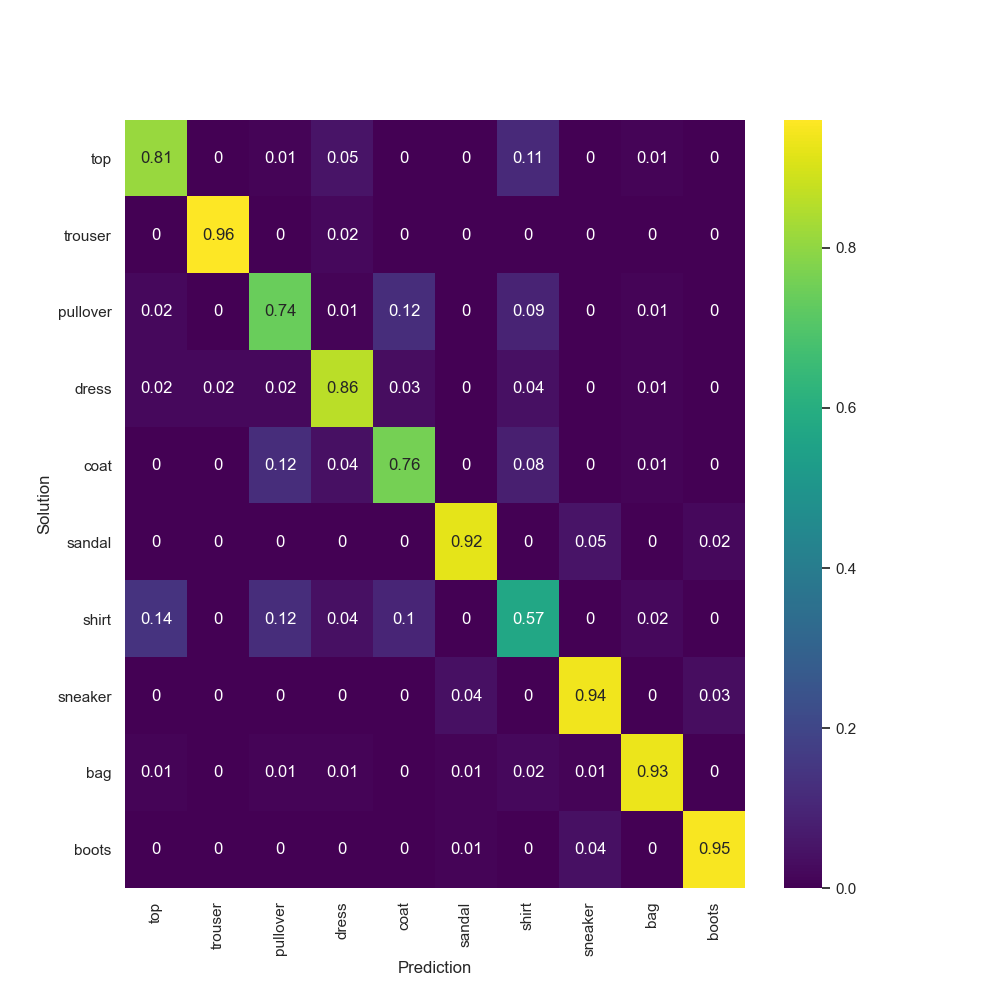
\includegraphics[width=0.8\textwidth]{assets/logreg_fashion_heatmap_accuracy84.png}
    \caption{The confusion matrix after using logistic regression to classify the fashion mnist. The matrix shows the accuracy of the model within each predicted class}
    \label{fig:logreg_mnist_cm}
\end{figure}

Some of the missclassified pictures from using logistic regression on the fashion mnist dataset can be seen in figure \ref{fig:missclassified_logreg_fashion}

\begin{figure}[H]
    \centering
    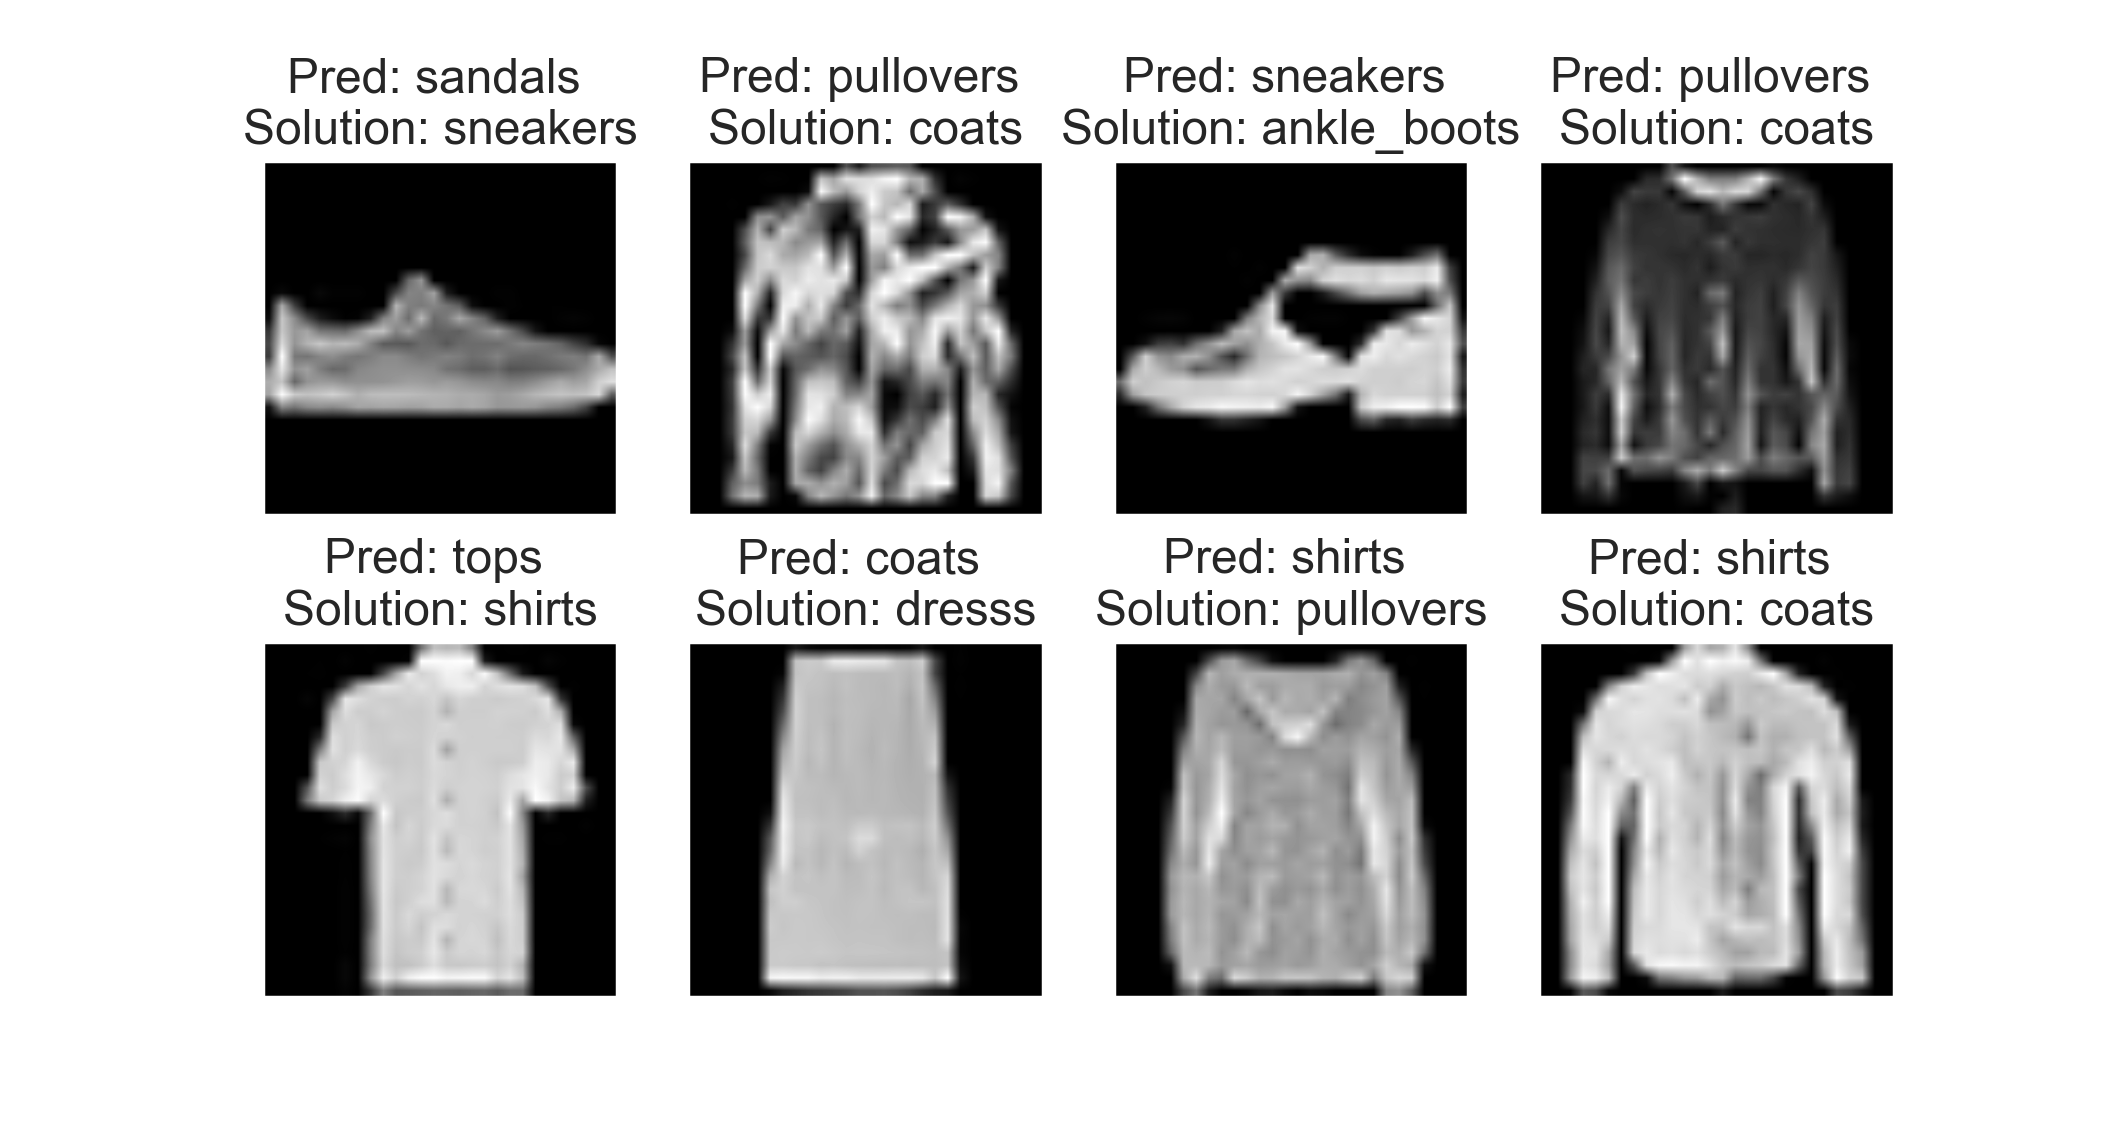
\includegraphics[width=0.8\textwidth]{assets/logreg_missclassified_fasion.png}
    \caption{Some missclassified images from the mnist fashion dataset, predicted by logistic regression}
    \label{fig:missclassified_logreg_fashion}
\end{figure}

\subsection{Face mask detection}
\subsubsection{CNN}
With fairly few training epochs done, the training session had a pretty consistently low loss and high accuracy throughout. The validation set shows the same progression, as shown in figure \ref{fig:facemasks_cnn_history}.

\begin{figure}[H]
    \begin{subfigure}{.5\textwidth}
        \centering
        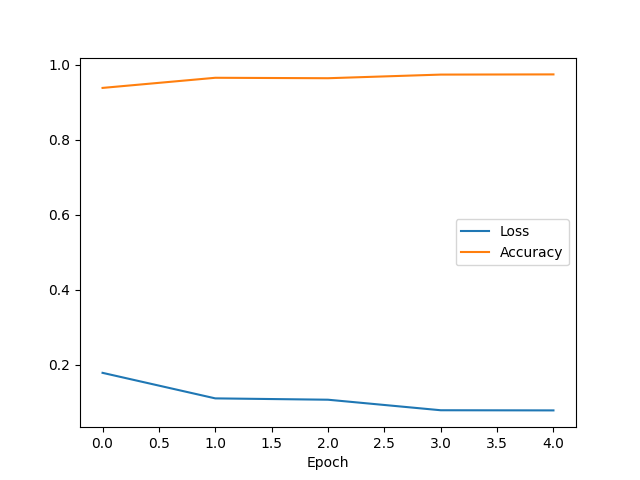
\includegraphics[width=1.1\linewidth]{assets/facemasks_train_history.png}
    \end{subfigure}
    \begin{subfigure}{.5\textwidth}
        \centering
        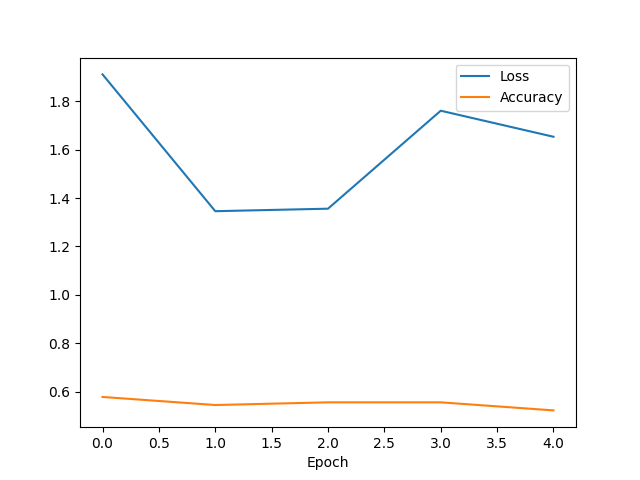
\includegraphics[width=1.1\linewidth]{assets/facemasks_val_history.png}
    \end{subfigure}
    \caption{History of loss and accuracy of the training and validation set as they develop through the epochs.}
    \label{fig:facemasks_cnn_history}
\end{figure}

After training on the training dataset, our model got an accuracy of approximately $98\%$ on the testing set. In addition to classifying the testing set, we snapped a couple of pictures of ourselves to test the network on. Figure \ref{fig:cnn_real_pics_predictions} shows some examples and the results the network provided.

\begin{figure}[H]
    \centering
    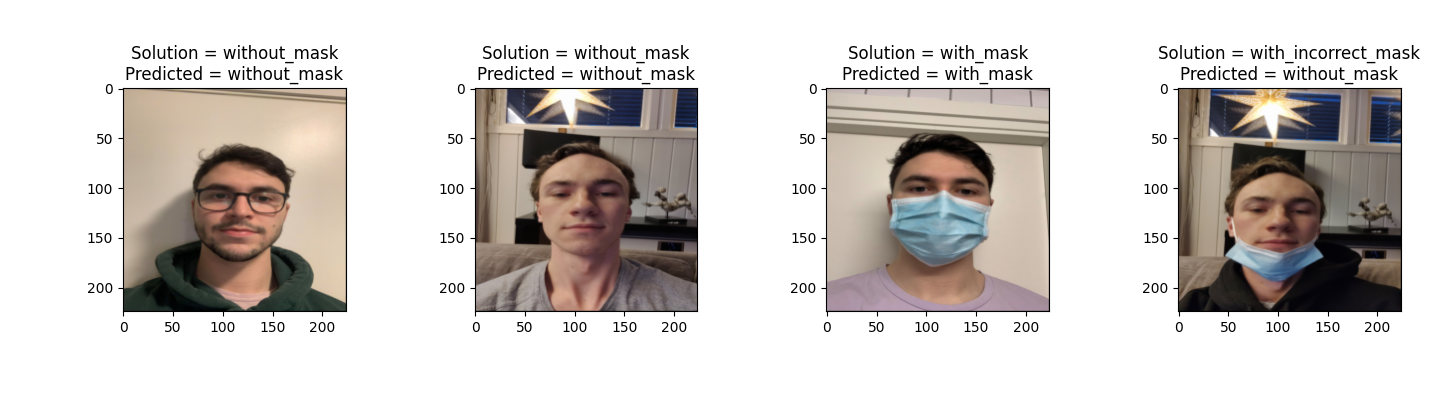
\includegraphics[width=\textwidth]{assets/cnn_real_pics_predictions.png}
    \caption{Pictures of ourselves and the predicted classifications of them.}
    \label{fig:cnn_real_pics_predictions}
\end{figure}


\subsubsection{Logistic regression}
The logistic regression model was applied on the face mask dataset. The logistic regression resulted with an accuracy score of 95\% when applied to the test set. The confusion matrix which shows the accuracy of the predicted classifications can be seen in figure \ref{fig:logreg_facemask_cm}. Some of the miss classified images can be seen in figure \ref{fig:missclassified_logreg_facemask}

\begin{figure}[H]
    \centering
    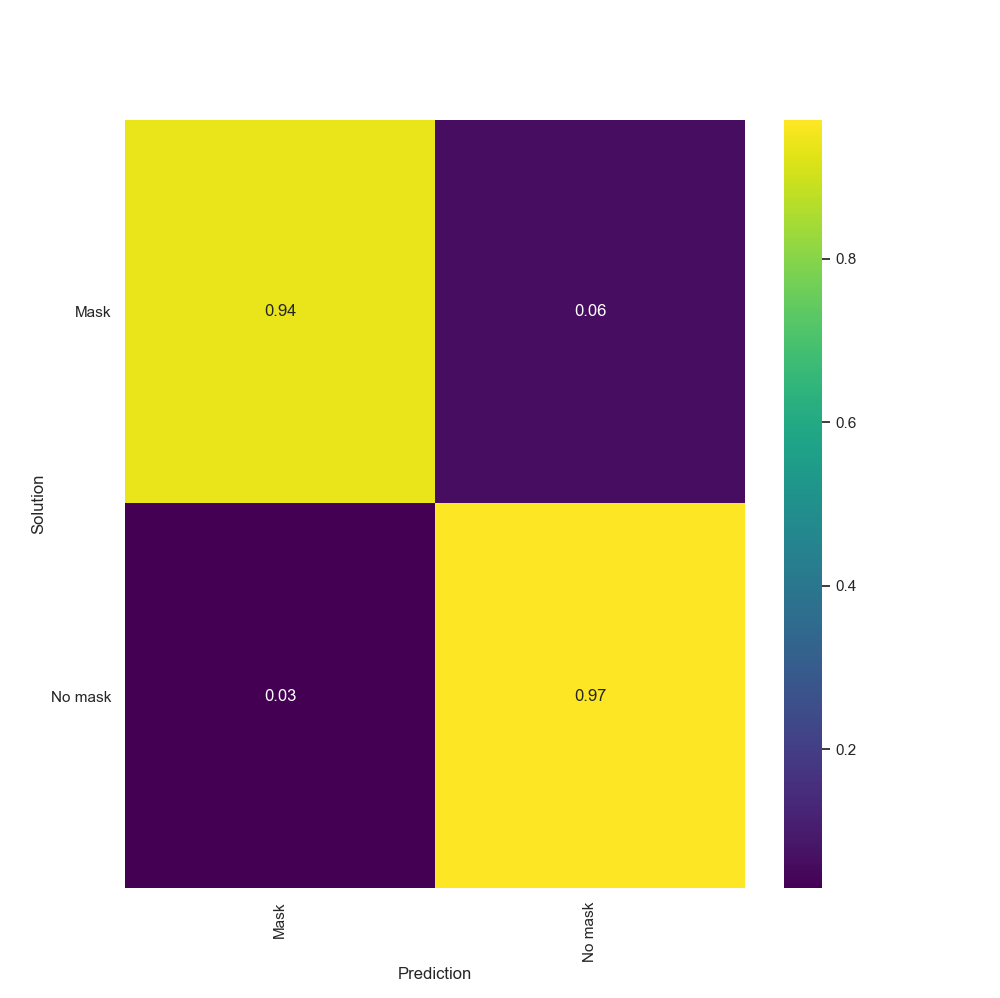
\includegraphics[width=0.8\textwidth]{assets/logreg_mask_heatmap_accuracy95.png}
    \caption{The confusion matrix after using logistic regression to classify the face mask detection dataset. The matrix shows the accuracy of the model within each predicted class}
    \label{fig:logreg_facemask_cm}
\end{figure}

\begin{figure}[H]
    \centering
    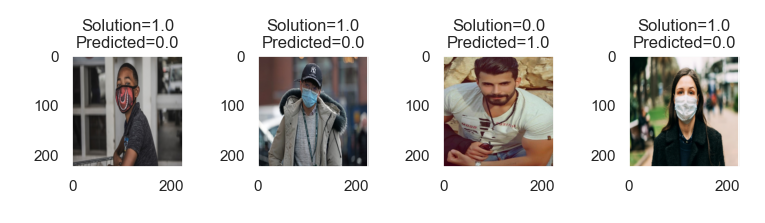
\includegraphics[width=1\textwidth]{assets/logreg_missclassified_facemask.png}
    \caption{Some miss classified images from the facemask detection dataset, predicted by logistic regression}
    \label{fig:missclassified_logreg_facemask}
\end{figure}


Since the dataset consisted of images of people with facemasks edited on instead of wearing real physical masks, the model was tested on a few pictures taken by ourself to check how the model performed after training. The results can be seen in figure \ref{fig:logreg_real_pics}

\begin{figure}[H]
    \centering
    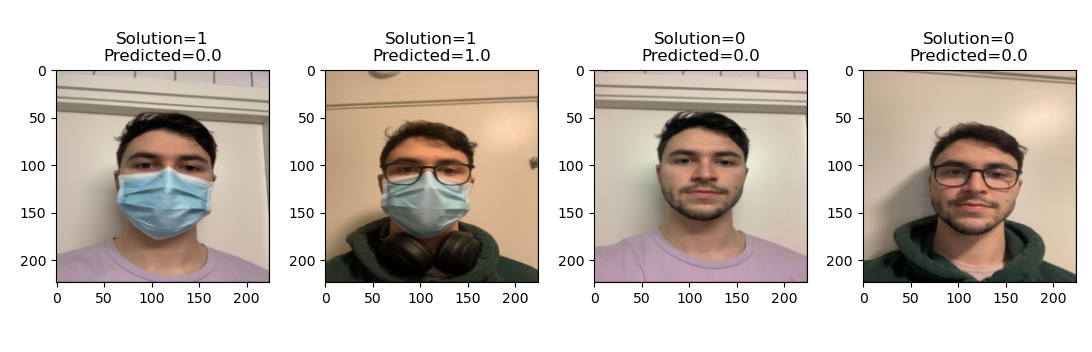
\includegraphics[width=1\textwidth]{assets/log_reg_real_pics.png}
    \caption{Pictures taken by ourselves to test the model. The model predicted three out of four pictures correct}
    \label{fig:logreg_real_pics}
\end{figure}


\end{document}